\documentclass[12pt,a4,oneside,usenames,dvipsnames]{book}
  \usepackage{polyglossia}
  \usepackage{fontspec}
  \setmainlanguage{english}
  \setotherlanguage{greek}
  \setmainfont[Scale=0.8]{Avara}
  \usepackage{unicode-math}
  %\setmathfont{Latin Modern Math}
  \setmathfont{TeX Gyre Pagella Math}
  \newfontfamily\pixel[Scale=1]{terminal-grotesque.ttf}
  \usepackage{microtype}
  \usepackage{dot2texi}
  \usepackage{hyperref}
\hypersetup{
    unicode,
    verbose=false,
    pdfpagelayout=TwoColumnRight,
    bookmarksopen,
    colorlinks,
    citecolor=black,
    filecolor=black,
    linkcolor=black,
    urlcolor=black
}
  \usepackage{microtype}
  \usepackage{amsmath}
  \usepackage{float}
  \usepackage{skeldoc}
  \floatplacement{figure}{H}
  \usepackage{tikz}
  \usepackage{svg}
  \usepackage{metalogo}
  \usepackage{csquotes}
  \usepackage[compact,nostruts,medium]{titlesec}
  %\titlespacing*{\chapter}{0pt}{0pt}{0pt}
  \newcommand\makeskelfig{%
  \begin{figure}
  {\centering%
  \skelfig[width=0.4\textwidth]{2\baselineskip}%
  \skelcaption[width=0.2\textwidth,lines=1]{}}
  \end{figure}}
  \usepackage{setspace}
  \usepackage{xcolor}
  \definecolor{bgcolor}{rgb}{0.95,0.95,0.95}
  \definecolor{red}{rgb}{1,0,0}
  \definecolor{gray}{RGB}{24,24,24}
   \definecolor{thered}    {rgb} {0.65,0.04,0.07}
 \definecolor{thegreen}  {rgb} {0.06,0.44,0.08}
 \definecolor{theblue}   {rgb} {0.02,0.04,0.48}
 \definecolor{sectioning}{gray}{0.44}
 \definecolor{thegrey}   {gray}{0.5}
 \definecolor{theframe}  {gray}{0.75}
 \definecolor{theshade}  {gray}{0.94}
\usepackage[cache=false,outputdir=build]{minted}
%\setminted[tex]{breaklines=true,linenos=true,bgcolor=theshade,frame=single,framesep=5pt,rulecolor=theframe}
%\setminted[shell]{breaklines=true,linenos=true,bgcolor=theshade,frame=single,framesep=5pt,rulecolor=theframe}
%\definecolor{bg}{rgb}{0.95,0.95,0.95}
\usepackage{xspace}
\usepackage{contour}
\usepackage[normalem]{ulem}
\usepackage{minted}
\usemintedstyle{bw}

\renewcommand{\ULdepth}{1.8pt}
\contourlength{0.8pt}

\newcommand\bitmap{{\pixel{}bitmap}}
\newcommand\colorunderline[1]{\bgroup\markoverwith{\textcolor{#1}{\rule[-0.5ex]{2pt}{0.8pt}}}\ULon}
\newcommand{\myuline}[2]{%
  \colorunderline{#1}{\phantom{#2}}%
  \llap{\contour{white}{#2}}%
}
\newcommand{\myurl}[2]{%
  \href{#1}{\myuline{blue}{#2}}%
}

\newcommand\titletext{A {\pixel{}Bitmapper}'s Geometry}
\title{\titletext{}}
\newcommand\subtitle{\emph{An introduction to basic bitmap mathematics and algorithms}}
\newcommand\biblatex{\texttt{biblatex}\xspace}%
\hypersetup{
  pdftitle={\titletext{}},
  pdfauthor={epilys},
  pdfsubject={programming},
}
\begin{document}
\setstretch{1.1}
\addtolength{\parskip}{5pt}%
\newlength\drop
\thispagestyle{empty}
\begingroup% Harry Carter
\setlength{\drop}{0.1\textheight}
\vspace*{\drop}
\begin{flushleft}
    \rule{\textwidth}{1.6pt}%
    \vspace{-0.9\baselineskip}
    \rule{\textwidth}{0.4pt}\\[0.8\baselineskip]
    {\centering
    \scalebox{2.0}{\parbox{0.5\textwidth}{\centering\Huge{}\textsc{{\titletext{}}}}}\\
    \vspace{1.5\baselineskip}
    {\LARGE\subtitle{}}\par
    \vspace*{0.3\baselineskip}
    }\rule{\textwidth}{1.6pt}%
    \vspace{-0.9\baselineskip}
    \rule{\textwidth}{0.4pt}\\[0.5\baselineskip]
    {\Large{}epilys}\hfill{\small{}\today{}}
\vfill%
\end{flushleft}%
\endgroup
\clearpage{}
This work is licensed under the Creative Commons Attribution-NonCommercial-ShareAlike 3.0 Unported License. To view a copy of this license, visit \url{http://creativecommons.org/licenses/by-nc-sa/3.0/} or send a letter to Creative Commons, PO Box 1866, Mountain View, CA 94042, USA.

The source code for this work is available under the GNU GENERAL PUBLIC LICENSE version 3 or later. You can view it, study it, modify it for your purposes as long as you respect the license if you choose to distribute your modifications.

The source code is available here

\url{https://github.com/epilys/bitmappers-geometry}

\tableofcontents
\chapter{Introduction}
The data structures we're going to use is \emph{Point} and \emph{Image}. \emph{Image} represents a \bitmap{}, although we will use full RGB colors for our points therefore the size of a pixel in memory will be \texttt{u8} instead of 1 bit.

\begin{minted}{rust}
pub type Point = (i64, i64);

pub const fn from_u8_rgb(r: u8, g: u8, b: u8) -> u32 {
    let (r, g, b) = (r as u32, g as u32, b as u32);
    (r << 16) | (g << 8) | b
}
pub const AZURE_BLUE: u32 = from_u8_rgb(0, 127, 255);
pub const RED: u32 = from_u8_rgb(157, 37, 10);
pub const WHITE: u32 = from_u8_rgb(255, 255, 255);
pub const BLACK: u32 = 0;

pub struct Image {
    pub bytes: Vec<u32>,
    pub width: usize,
    pub height: usize,
    pub x_offset: usize,
    pub y_offset: usize,
}

impl Image {
    pub fn new(width: usize,
        height: usize,
        x_offset: usize,
        y_offset: usize) -> Self;
    pub fn draw(&self,
        buffer: &mut Vec<u32>,
        fg: u32,
        bg: Option<u32>,
        window_width: usize);
    pub fn draw_outline(&mut self);
    pub fn clear(&mut self);
    pub fn plot(&mut self, x: i64, y: i64);
    pub fn get(&mut self, x: i64, y: i64) -> u32;
    pub fn plot_ellipse(
        &mut self,
        (xm, ym): (i64, i64),
        (a, b): (i64, i64),
        quadrants: [bool; 4],
        _wd: f64,
    );
    pub fn plot_line_width(&mut self,
              point_a: Point,
              point_b: Point,
              wd: f64);
    pub fn flood_fill(&mut self, mut x: i64, y: i64);
}
\end{minted}

A way to display an \emph{Image} is to use the \texttt{minifb} crate which allows you to create a window and draw pixels directly on it. Here's how you could set it up:

\begin{minted}{rust}
use bitmappers_geometry::*;
use minifb::{Key, Window, WindowOptions};

const WINDOW_WIDTH: usize = 400;
const WINDOW_HEIGHT: usize = 400;

fn main() {
    let mut buffer: Vec<u32> = vec![WHITE; WINDOW_WIDTH * WINDOW_HEIGHT];
    let mut window = Window::new(
        "Test - ESC to exit",
        WINDOW_WIDTH,
        WINDOW_HEIGHT,
        WindowOptions {
            title: true,
            //borderless: true,
            //resize: false,
            //transparency: true,
            ..WindowOptions::default()
        },
    )
    .unwrap();

    // Limit to max ~60 fps update rate
    window.limit_update_rate(Some(std::time::Duration::from_micros(16600)));

    let mut image = Image::new(50, 50, 150, 150);
    image.draw_outline();
    image.draw(&mut buffer, BLACK, None, WINDOW_WIDTH);

    while window.is_open()
         && !window.is_key_down(Key::Escape)
         && !window.is_key_down(Key::Q) {
        window
            .update_with_buffer(&buffer, WINDOW_WIDTH, WINDOW_HEIGHT)
            .unwrap();
        let millis = std::time::Duration::from_millis(100);
        std::thread::sleep(millis);
    }
}
\end{minted}

Running this will show you something like this:

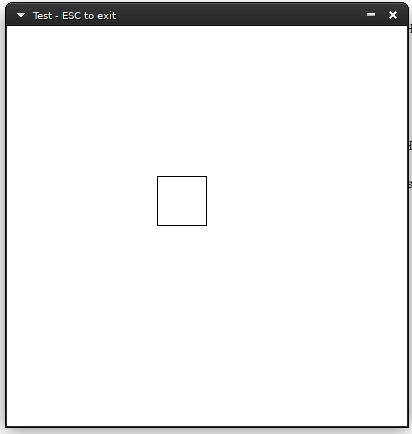
\includegraphics{figures/introduction.png}

\section{Loading \texttt{xbm} files in Rust}

\texttt{xbm} files are C source code files that contain the pixel information for an image as macro definitions for the dimensions and a static \texttt{char} array for the pixels, with each bit column representing a pixel. If the width dimension doesn't have 8 as a factor, the remaining bit columns are left blank/ignored.

They used to be a popular way to share user avatars in the old internet and are also good material for us to work with, since they are small and numerous. The following is such an image:

\begin{center}

\includegraphics{figures/news.png}
\end{center}

First, let's define a way to convert bit information to a byte vector:

\begin{minted}{rust}
pub fn bits_to_bytes(bits: &[u8], width: usize) -> Vec<u32> {
    let mut ret = Vec::with_capacity(bits.len() * 8);
    let mut current_row_count = 0;
    for byte in bits {
        for n in 0..8 {
            if byte.rotate_right(n) & 0x01 > 0 {
                ret.push(BLACK);
            } else {
                ret.push(WHITE);
            }
            current_row_count += 1;
            if current_row_count == width {
                current_row_count = 0;
                break;
            }
        }
    }
    ret
}
\end{minted}

Then, we can convert the \texttt{xbm} file from C to Rust with the following transformations:

\begin{minted}{c}
#define news_width 48
#define news_height 48
static char news_bits[] = {
\end{minted}

to


\begin{minted}{rust}
const NEWS_WIDTH: usize = 48;
const NEWS_HEIGHT: usize = 48;
const NEWS_BITS: &[u8] = &[
\end{minted}

And replace the closing \texttt{\}} with \texttt{]}.

We can then include the new file in our source code:


\begin{minted}{rust}
include!("news.xbm.rs");
\end{minted}

load the image:

\begin{minted}{rust}
let mut image = Image::new(NEWS_WIDTH, NEWS_HEIGHT, 25, 25);
image.bytes = bits_to_bytes(NEWS_BITS, NEWS_WIDTH);
\end{minted}

and finally run it:

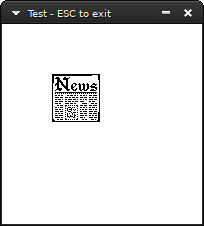
\includegraphics{figures/intro-2.png}

\part{Points and Lines}
\chapter{Distance between two points}

\begin{center}
\input{fig1.pdf_tex}
\end{center}

Given two points, $K$ and $L$, an elementary application of Pythagoras' Theorem gives the distance between them as

\begin{equation}
  r = \sqrt{(x_{L} - x_{K})^{2} +(y_{L} - y_{K})^{2}}
\end{equation}

which is simply coded:

\begin{minted}{rust}
pub fn distance_between_two_points(p_k: Point, p_l: Point) -> f64 {
    let (x_k, y_k) = p_k;
    let (x_l, y_l) = p_l;
    let xlk = x_l - x_k;
    let ylk = y_l - y_k;
    f64::sqrt((xlk*xlk + ylk*ylk) as f64)
}
\end{minted}

\section{Drawing a line segment from its two endpoints}

For any line segment with any slope, pixels must be matched with the infinite
amount of points contained in the segment. As shown in the following figure, a segment \emph{touches} some pixels; we could fill them using an algorithm and get a \bitmap{} of the line segment.

\begin{center}
\input{fig2.pdf_tex}
\end{center}

The algorithm presented here was first derived by Bresenham. In the \emph{Image} implementation, it is used in the \texttt{plot\_line\_width} method.
%\begin{minted}{rust}
%    pub fn plot_line_width(&mut self,
%                       (mut x0, mut y0): (i64, i64),
%                       (x1, y1): (i64, i64),
%                       wd: f64) {
%        /* Bresenham's line algorithm */
%        let dx = (x1 - x0).abs();
%        let sx = if x0 < x1 { 1 } else { -1 };
%        let dy = (y1 - y0).abs();
%        let sy = if y0 < y1 { 1 } else { -1 };
%        let mut err = dx - dy;
%        /* error value e_xy */
%        let mut e2: i64;
%        let mut x2: i64;
%        let mut y2: i64;
%        let ed: f64 = if (dx + dy) == 0 {
%            1.0
%        } else {
%            f64::sqrt((dx * dx) as f64 + (dy * dy) as f64)
%        };
%        let mut points = vec![];
%        let wd = (wd + 1.0) / 2.0;
%        //eprintln!("wd = {}, ed = {}", wd, ed);
%        loop {
%            points.push((x0, y0));
%            self.plot(x0, y0);
%            e2 = err;
%            x2 = x0;
%            if 2 * e2 >= -dx {
%                /* x step */
%                //eprintln!(" x step ");
%                e2 += dy;
%                y2 = y0;
%                while e2 < ((ed as f64 * wd) as i64)
%                       && (y1 != y2 || dx > dy) {
%                    y2 += sy;
%                    self.plot(x0, y2);
%                    points.push((x0, y2));
%                    e2 += dx;
%                }
%                if x0 == x1 {
%                    break;
%                };
%                e2 = err;
%                err -= dy;
%                x0 += sx;
%            }
%            if 2 * e2 <= dy {
%                /* y step */
%                //eprintln!(" y step ");
%                e2 = dx - e2;
%                while e2 < ((ed as f64 * wd) as i64)
%                       && (x1 != x2 || dx < dy) {
%                    x2 += sx;
%                    self.plot(x2, y0);
%                    points.push((x2, y0));
%                    e2 += dy;
%                }
%                if y0 == y1 {
%                    break;
%                };
%                err += dx;
%                y0 += sy;
%            }
%        }
%    }
%\end{minted}


\chapter{Equations of a line}
\chapter{The parametric form}
\chapter{Angle between two lines}
\chapter{Intersection of two lines}
\chapter{Line through two points}
\chapter{Line equidistant from two points}
\chapter{Normal to a line through a point}
\part{Points Lines and Circles}
\chapter{Equations of a Circle}
\part{Points line segments and Arcs}
\part{Curves other than circles}
\part{Points, lines and planes}
\part{Vectors, matrices and transformations}
\chapter{Rotation of a \bitmap{}}

\[
  p' =
  \begin{bmatrix}
    cosθ & -sinθ\\
    sinθ & cosθ
  \end{bmatrix} \]\[ \begin{bmatrix}
    x_{p}\\
    y_{p}
  \end{bmatrix}
\]

\begin{equation*}
  c = cosθ,\\\\
  s = sinθ,\\
  x_{p'} = x_{p}c-y_{p}s,\\
  y_{p'} = x_{p}s+y_{p}c.
\end{equation*}

Let's load an \texttt{xface}. We will use \texttt{bits\_to\_bytes} (See Introduction).

\begin{minted}{rust}
include!("dmr.rs");

const WINDOW_WIDTH: usize = 100;
const WINDOW_HEIGHT: usize = 100;

let mut image = Image::new(DMR_WIDTH, DMR_HEIGHT, 25, 25);
image.bytes = bits_to_bytes(DMR_BITS, DMR_WIDTH);
\end{minted}

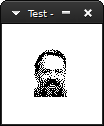
\includegraphics{figures/ch11-1.png}

This is the \texttt{xface} of \texttt{dmr}. Instead of displaying the \bitmap{}, this time we will rotate it $0.5$ radians. Setup our image first:


\begin{minted}{rust}
let mut image = Image::new(DMR_WIDTH, DMR_HEIGHT, 25, 25);
image.draw_outline();
let dmr = bits_to_bytes(DMR_BITS, DMR_WIDTH);
\end{minted}

And then, loop for each byte in \texttt{dmr}'s face and apply the rotation transformation.

\begin{minted}{rust}
let angle = 0.5;

let c = f64::cos(angle);
let s = f64::sin(angle);

for y in 0..DMR_HEIGHT {
    for x in 0..DMR_WIDTH {
        if dmr[y * DMR_WIDTH + x] == BLACK {
            let x = x as f64;
            let y = y as f64;
            let xr = x * c - y * s;
            let yr = x * s + y * c;
            image.plot(xr as i64, yr as i64);
        }
    }
}
\end{minted}

The result:

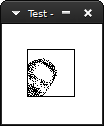
\includegraphics{figures/ch11-2.png}

We didn't mention in the beginning that the rotation has to be relative to a \emph{point} and the given transformation is relative to the \emph{origin}, in this case the upper left corner $(0,0)$. Usually, we want to rotate something relative to itself. The right point to choose is the \emph{centroid} of the object.

If we have a list of $n$ points, the centroid is calculated as:

$$ x_c = \frac{1}{n}\sum_{i=0}^{n} x_i $$
$$ y_c = \frac{1}{n}\sum_{i=0}^{n} y_i $$

Since in this case we have a rectangle, the centroid has coordinates of half the width and half the height.

By subtracting the centroid from each point before we apply the transformation and then adding it back after we get what we want:

\begin{minted}{rust}
let center_point = ((DMR_WIDTH/2) as i64, (DMR_HEIGHT/2) as i64);
for y in 0..DMR_HEIGHT {
    for x in 0..DMR_WIDTH {
        if dmr[y * DMR_WIDTH + x] == BLACK {
            let x = (x as i64 -center_point.0) as f64;
            let y = (y as i64 -center_point.1) as f64;
            let xr = x * c - y * s;
            let yr = x * s + y * c;
            image.plot(xr as i64+center_point.0,
                       yr as i64 + center_point.1);
        }
    }
}
\end{minted}

The result:

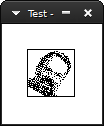
\includegraphics{figures/ch11-3.png}

\chapter{Rotation of a \bitmap{} by parallel recusive subdivision}
\chapter{Magnification}
\part{Flood filling}
\part{Areas}
\part{Volumes}
\skelpars{3}
\end{document}
